\documentclass[tikz,border=8pt]{standalone}
% Shared look for every TikZ diagram. Load with \input{../../tools/tikz-style.tex}
\usepackage[T1]{fontenc}
\usepackage{lmodern}
\renewcommand{\sfdefault}{lmr}  % diagrams use the same serif as the text
\usetikzlibrary{arrows.meta, positioning, shapes.geometric, calc, fit, backgrounds}
\definecolor{cblue}{HTML}{4C78A8}
\definecolor{corange}{HTML}{F58518}
\definecolor{cgreen}{HTML}{54A24B}
\definecolor{cred}{HTML}{E45756}
\definecolor{cpurple}{HTML}{B279A2}
\definecolor{cgrey}{HTML}{6B6B6B}
\tikzset{
  every picture/.style={font=\sffamily, line width=1.2pt},
  box/.style={draw=#1, fill=#1!12, rounded corners=4pt, align=center, inner sep=7pt, minimum height=1.1cm},
  box/.default=cgrey,
  arrow/.style={-{Stealth[length=3mm]}, draw=cgrey, line width=1.4pt},
  title/.style={font=\sffamily\bfseries\Large},
  note/.style={font=\sffamily\small, text=cgrey, align=center},
}
\AtBeginDocument{\hyphenpenalty=10000 \exhyphenpenalty=10000}

\begin{document}
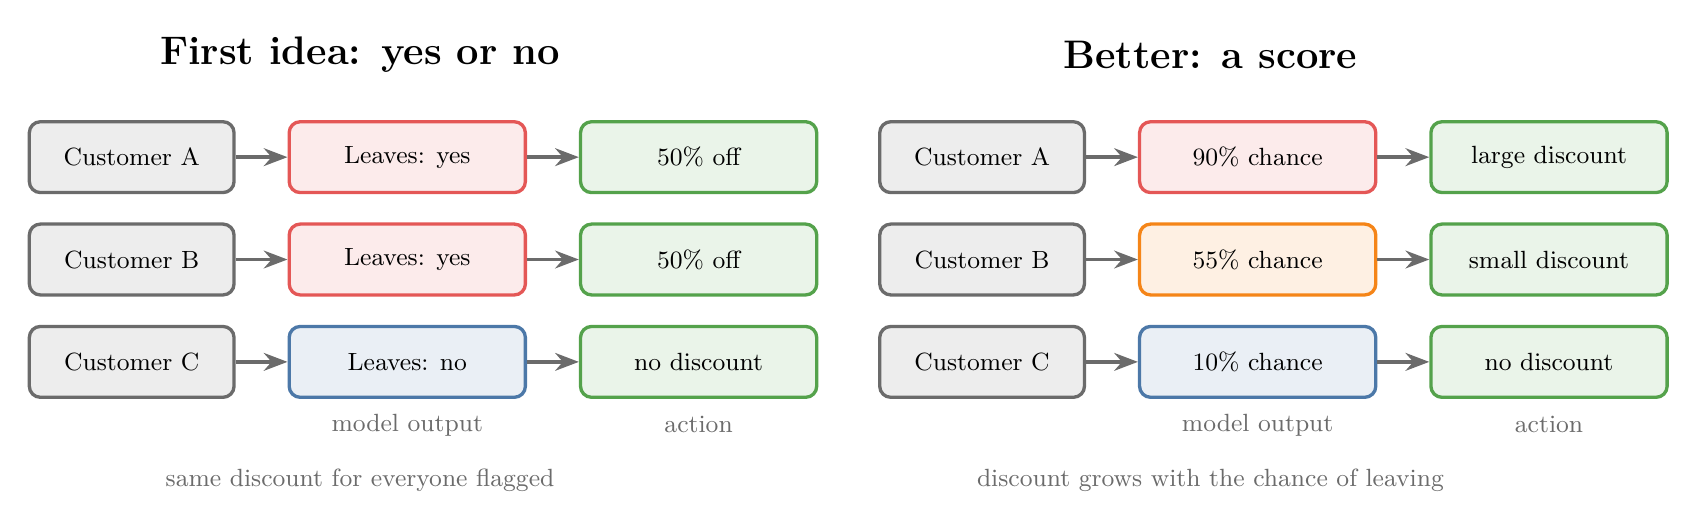
\begin{tikzpicture}
  \tikzset{
    cust/.style={box=cgrey, minimum width=2.6cm, minimum height=0.9cm, font=\small},
    out/.style={box=#1, minimum width=3.0cm, minimum height=0.9cm, font=\small},
    disc/.style={box=cgreen, minimum width=3.0cm, minimum height=0.9cm, font=\small},
  }
  % Left: first idea, yes / no
  \node[title] at (2.9,1.3) {First idea: yes or no};
  \foreach \n/\o/\d/\c [count=\i] in {A/Leaves: yes/50\% off/cred, B/Leaves: yes/50\% off/cred, C/Leaves: no/no discount/cblue}{
    \node[cust] (l\i) at (0,-1.3*\i+1.3) {Customer \n};
    \node[out=\c] (lo\i) at (3.5,-1.3*\i+1.3) {\o};
    \node[disc] (ld\i) at (7.2,-1.3*\i+1.3) {\d};
    \draw[arrow] (l\i) -- (lo\i);
    \draw[arrow] (lo\i) -- (ld\i);
  }
  % Right: better idea, a score
  \begin{scope}[xshift=10.8cm]
  \node[title] at (2.9,1.3) {Better: a score};
  \foreach \n/\o/\d/\c [count=\i] in {A/90\% chance/{large discount}/cred, B/55\% chance/{small discount}/corange, C/10\% chance/no discount/cblue}{
    \node[cust] (r\i) at (0,-1.3*\i+1.3) {Customer \n};
    \node[out=\c] (ro\i) at (3.5,-1.3*\i+1.3) {\o};
    \node[disc] (rd\i) at (7.2,-1.3*\i+1.3) {\d};
    \draw[arrow] (r\i) -- (ro\i);
    \draw[arrow] (ro\i) -- (rd\i);
  }
  \end{scope}
  \node[note] at (3.5,-3.4) {model output};
  \node[note] at (7.2,-3.4) {action};
  \node[note] at (14.3,-3.4) {model output};
  \node[note] at (18.0,-3.4) {action};
  \node[note] at (2.9,-4.1) {same discount for everyone flagged};
  \node[note] at (13.7,-4.1) {discount grows with the chance of leaving};
\end{tikzpicture}
\end{document}
